
\documentclass[preprint,12pt,a4]{standalone}
\usepackage{geometry}   % my added package "geometry"
\geometry{letterpaper,tmargin=1in,bmargin=1in,lmargin=2.5cm,rmargin=2.5cm}
\usepackage{tikz}
\usetikzlibrary{calc,patterns,arrows.meta,shapes.arrows,intersections,positioning}
\usetikzlibrary{decorations.pathmorphing,backgrounds,fit,petri}
\usepackage{standalone}
\begin{document}
	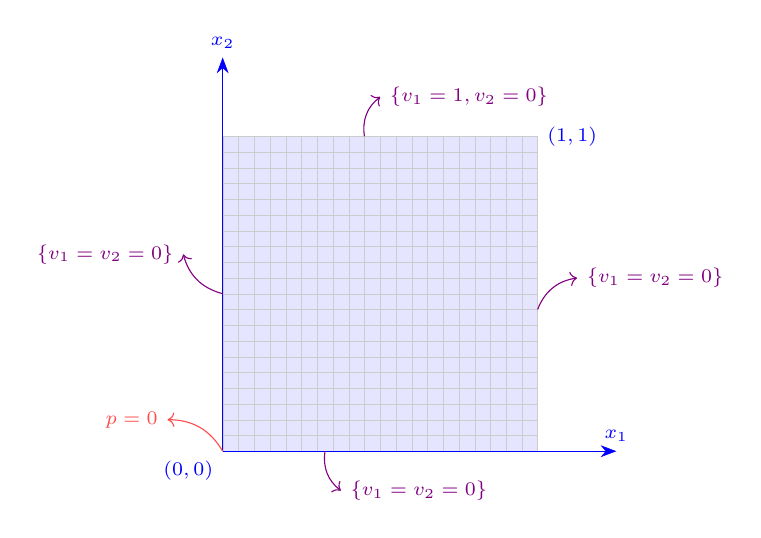
\begin{tikzpicture} [{place/.style={rectangle,draw=blue!50,fill=blue!20,ultra thin,inner sep=0.8mm}},{place2/.style={circle,draw=black!50,ultra thin,inner sep=0.8mm}},{linest/.style={color=gray,ultra thin}}]
	%%coordinates of corners of Beam
	\coordinate (A) at (0,0);
	\coordinate (B) at (4.0,0);
	\coordinate (D) at (4.0,4.0);
	\coordinate (E) at (0.0,4.0);
	
	%% fluid
	\draw [gray!30,fill=blue!10](A) rectangle (D)node [right,color = blue,font=\scriptsize] {$(1,1)$};
	%%mesh
	\draw [line width=0.1pt,gray!40,step=2mm](0,0) grid (D);

	%%axes
	\draw [-{Stealth[length=2mm]},help lines,blue] ($(0,0)$)node [below left,color = blue,font=\scriptsize] {$(0,0)$} -> ($(B)+(1,0)$) node [above,color = blue,font=\scriptsize] {$x_1$};
	\draw [-{Stealth[length=2mm]}, help lines,blue] ($(0,0)$) -> ($(D)+(-4,1)$) node [above,color = blue,font=\scriptsize] {$x_2$};
	

	%%BC
	%% velocity
	\draw [->,violet] (4,1.8) to [bend left] (4.5,2.2)node [right,color = violet,font=\scriptsize] {\{$v_1=v_2=0\}$};
	
	\draw [->,violet] (1.8,4) to [bend left] (2.0,4.5)node [right,color = violet,font=\scriptsize] {\{$v_1=1, v_2=0\}$};
	
	\draw [->,violet] (0,2.0) to [bend left] (-0.5,2.5)node [left,color = violet,font=\scriptsize] {\{$v_1=v_2=0\}$};
	
	\draw [->,violet] (1.3,0) to [bend right] (1.5,-0.5)node [right,color = violet,font=\scriptsize] {\{$v_1=v_2=0\}$};
	%% pressure
	\draw [->,red!70] (0.0,0.0) to [bend right] (-0.7,0.4)node [left,color = red!70,font=\scriptsize] {$p=0$};
	\end{tikzpicture}
\end{document}